\subsection{Sintern}

\begin{table}[H]
\centering

\adjustbox{max width=\textwidth}{

% Resize the table to fit within the page
%\resizebox{\textwidth}{!}{%


\renewcommand{\arraystretch}{1.7} % Increase row height (local)
\fontsize{18pt}{20pt}\selectfont
\begin{tabular}{|l|c|c|c|c|}
\hline
\textbf{Scherkörper} & \multicolumn{1}{l|}{\textbf{Maximale Scherkraft} {[}\si{\newton}{]}} & \multicolumn{1}{l|}{\textbf{Durchschnittskraft} {[}\si{\newton}{]}} & \multicolumn{1}{l|}{\textbf{Fläche} {[}\si{\milli\meter\squared}{]}} & \multicolumn{1}{l|}{\textbf{Scherfestigkeit} {[}\si{\newton\per\milli\meter\squared}{]}} \\ \hline
\textbf{1} & 330,45 & 143,11 & 5,29 & 62,47 \\ \hline
\textbf{2} & 459,23 & 137,78 & 5,29 & 86,81 \\ \hline
\textbf{3} & 420,47 & 135,23 & 5,29 & 79,48 \\ \hline
\textbf{4} & 384,35 & 148,57 & 5,29 & 72,66 \\ \hline
\textbf{5} & 508,97 & 172,81 & 5,29 & 96,21 \\ \hline
\textbf{6} & 358,84 & 116,34 & 5,29 & 67,83 \\ \hline
\textbf{7} & 388,41 & 143,01 & 5,29 & 73,42 \\ \hline
\textbf{8} & 354,98 & 140,97 & 5,29 & 67,10 \\ \hline
\end{tabular}}
\vspace{0.5cm}
\caption{Sintern}
\label{Tab.1}
\end{table}




\begin{table}[H]
\centering

\adjustbox{max width=\textwidth}{

% Resize the table to fit within the page
%\resizebox{\textwidth}{!}{%


\renewcommand{\arraystretch}{1.7} % Increase row height (local)
\fontsize{18pt}{20pt}\selectfont
\begin{tabular}{|l|c|c|c|c|}
\hline
\textbf{Scherkörper} & \multicolumn{1}{l|}{\textbf{Maximale Scherkraft} {[}\si{\newton}{]}} & \multicolumn{1}{l|}{\textbf{Durchschnittskraft} {[}\si{\newton}{]}} & \multicolumn{1}{l|}{\textbf{Fläche} {[}\si{\milli\meter\squared}{]}} & \multicolumn{1}{l|}{\textbf{Scherfestigkeit} {[}\si{\newton\per\milli\meter\squared}{]}} \\ \hline
\textbf{1} & 195,05 & 77,34 & 5,29 & 36,87 \\ \hline
\textbf{2} & 146,72 & 55,16 & 5,29 & 27,74 \\ \hline
\textbf{3} & 143,32 & 47,98 & 5,29 & 27,09 \\ \hline
\textbf{4} & 129,39 & 39,87 & 5,29 & 24,46 \\ \hline
\textbf{5} & 142,67 & 54,48 & 5,29 & 26,97 \\ \hline
\textbf{6} & 128,16 & 51,59 & 5,29 & 24,23 \\ \hline
\textbf{7} & 147,18 & 70,87 & 5,29 & 27,82 \\ \hline
\textbf{8} & 131,37 & 49,35 & 5,29 & 24,83 \\ \hline
\textbf{9} & 175,58 & 78,33 & 5,29 & 33,19 \\ \hline
\end{tabular}}
\vspace{0.5cm}
\caption{Laminiert}
\label{Tab.2}
\end{table}





\begin{figure}[H]
    \centering
    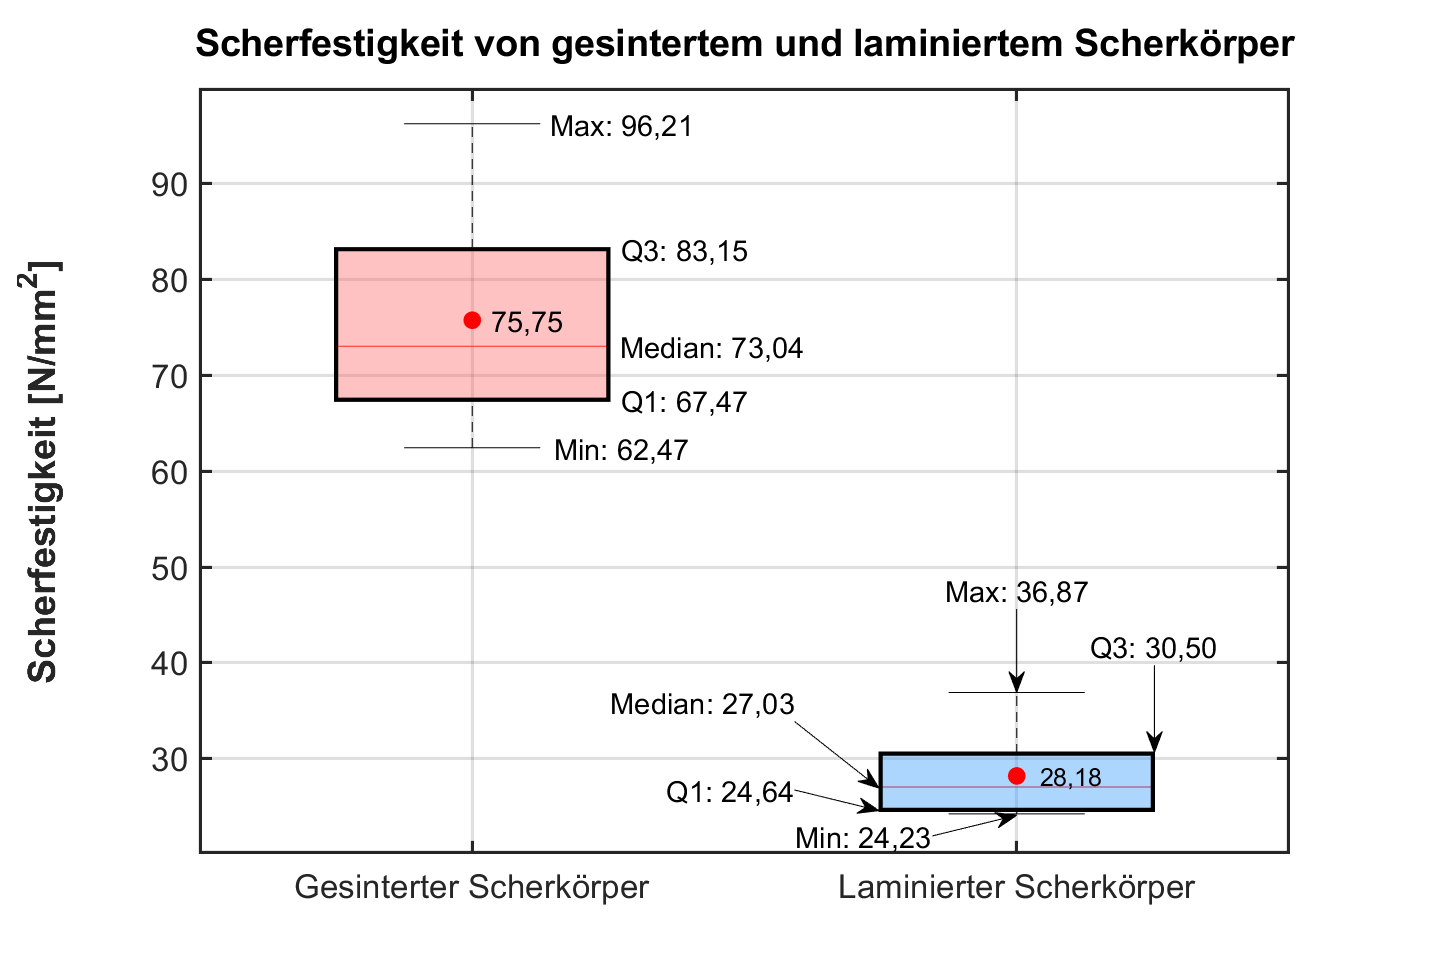
\includegraphics[width=0.7\textwidth]{Bilder/boxplot_final.eps}
    \caption{Boxplot der Scherfestigkeit {[}N/mm$^2${]} von gesinterten und laminierten Scherkörpern.}
    \label{fig:boxplot}
\end{figure}




